\documentclass{article}
\usepackage[utf8]{inputenc}
\usepackage{todonotes}
\usepackage{graphicx}
\usepackage{amsfonts}
\usepackage{amsmath}
\usepackage{hyperref}
\usepackage{cite}
\usepackage{listings}
\usepackage{color}

\definecolor{codegreen}{rgb}{0,0.6,0}
\definecolor{codegray}{rgb}{0.5,0.5,0.5}
\definecolor{codepurple}{rgb}{0.58,0,0.82}
\definecolor{backcolour}{rgb}{0.95,0.95,0.92}
 
\lstdefinestyle{mystyle}{
    backgroundcolor=\color{backcolour},   
    commentstyle=\color{codegreen},
    keywordstyle=\color{magenta},
    numberstyle=\tiny\color{codegray},
    stringstyle=\color{codepurple},
    basicstyle=\footnotesize,
    breakatwhitespace=false,         
    breaklines=true,                 
    captionpos=b,                    
    keepspaces=true,                 
    numbers=left,                    
    numbersep=5pt,                  
    showspaces=false,                
    showstringspaces=false,
    showtabs=false,                  
    tabsize=2
}

\lstset{style=mystyle}

\title{Integer factorization}
\author{Bastian Fredriksson \texttt{bastianf@kth.se}\\Fabian Ström \texttt{fabstr@kth.se}}
\date{December 2015}

\begin{document}

\maketitle
\newpage

\tableofcontents
\newpage

\section{Introduction}
Integer factorization of a composite number $N$ is the problem of finding a prime factor $p$ such that $p \mid N$. The integer factorization decision problem, is the problem of determining whether $N$ has a prime factor $p$ in the interval $1 < p \le M$ for some $M < N$. It is not known exactly to which complexity class this problem belongs, but it is known to be in both \textit{NP}, \textit{co-NP} and \textit{BQP}. 

An important open problem in computer science is whether there exists a polynomial time algorithm for the integer factorization problem running on a conventional computer. Any such algorithm would effectively render the RSA encryption algorithm insecure, which relies on the hardness of  integer factorization. The best known algorithms for integer factorization is running in sub-exponential time, making integer factorization intractable for composite numbers with only large prime factors. The best known algorithms are the \textit{General Field Sieve algorithm (GFNS)}, the \textit{Quadratic Sieve algorithm (QS)} and \textit{Lenstra's elliptic curve factorization algorithm}, also known as the \textit{Elliptic Curve Method (ECM)}. 

\section{Overview}
In this report we describe the algorithms used to create a program which specializes in factorization of integers with $\leq 29$ digits.

We have used Sphere Online Judge (SPOJ) to test the robustness of our integer factorization program. The SPOJ tests are divided into three separate tests known as FACT0, FACT1 and FACT2. The FACT0 test is the easiest and contains composites up to 15 digits. The FACT1 test is somewhat harder and contains composites up to 20 digits. The hardest test is FACT2, which contains composites up to 29 digits. All tests contains about 10 composites to factor and must finish in 2 seconds. 

Our SPOJ program is written in Java and uses three different algorithms for factorization. It has been successfully benchmarked against both the FACT1 and FACT2 tests, and is at the time of writing the fastest Java implementation, even on par with some C++ implementations.

We use trial division with a precomputed table of small primes to quickly break out the smallest factors. Pollard Rho with Brent's cycle detection is used for composites not exceeding $\sqrt{2^{63}-3}$. For any larger composite, Shank's Square Forms Factorization (SQUFOF) is used. 

The consequence of this is that almost all calculations are carried out using 64-bit integers. Pollard Rho is discussed in section \ref{pollard} and SQUFOF is discussed in section \ref{squfof}.

To determine if a factor is prime, we use a randomised Miller-Rabbin primality test with 20 rounds. Miller-Rabbin is briefly mentioned in section \ref{primetest}. 

For an overview of the complete implementation of the factorization algorithm, see figure \ref{fig:flowchart}.

We have also implemented The Elliptic Curve Method, which is discussed in section \ref{ecm}. The implementation is multithreaded, written in C and uses GMP for large integer arithmetic. The implementation has not been tested on SPOJ, but offline tests on composites up to 50 digits have been conducted, with good results (the number was factorized within a few minutes). 

\begin{figure}[p!]
\centering
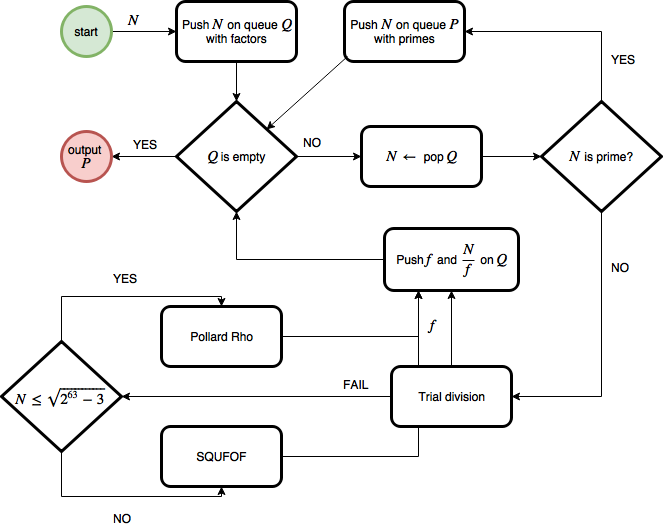
\includegraphics[width=\textwidth]{flowchart}
\caption{Flowchart for an integer factorisation circuit constructed using a primality test, Pollard Rho, SQUFOF and trial division. The numbers being processed are stored in two queues, one queue $Q$ containing numbers to be factored, and one queue $P$ with primes. The algorithm terminates when $Q$ is empty, yielding the complete factorisation of $N$.}
\label{fig:flowchart}
\end{figure}

\newpage
\lstinputlisting[language=C]{factor.c}


\section{Elliptic curve method}
\label{ecm}
Lenstra's elliptic curve factorization algorithm or the elliptic curve method (ECM) is the third fastest algorithm for general integer factorization with an expected worst-case running time of $O(e^{\sqrt{\log n \log\log n}})$\cite{Lenstra87}. Similar to Pollard Rho, the running time of ECM is proportional to the size of the smallest prime factor. This makes ECM suitable for finding small prime factors up to 25 digits before switching to another algorithm such as the Quadratic Sieve. The algorithm is based on finite field arithmetics over elliptic curves.

ECM starts by selecting a smooth elliptic curve, and a point $P$ on the curve randomly. The next step is to perform repeated addition $eP$ over $\mathbb{Z}_N$ where $N$ is the composite number to be factored. The integer $e$ should be chosen as a number containing powers of many small prime numbers. The algorithm proceeds until a non-invertible element $x$ in $\mathbb{Z}_N$ is detected, which yields a prime factor of $N$ as $gcd(x, N)$. A new elliptic curve and point is selected if $e$ becomes large or if $eP=\mathcal{O}$.
\\\\
Here follows a description of the first phase of our implementation in more detail.
\begin{enumerate}
\item \textbf{Selection of the elliptic curve and curve point} Pick an elliptic curve described by the Weierstrass equation $y^2 = x^3 + ax + b$ by selecting a non-trivial point $P=(x_0, y_0)$ and $a$ randomly from $\mathbb{Z}_N$. Calculate $b = y_0^2-x_0^3-ax_0$. Repeat this process until a smooth elliptic curve is found, that is a curve such that $-4a^3-27b^2\ne_N 0$\cite{Silverman93}.

\item \textbf{Perform repeated addition over $\mathbb{Z}_N$}. Calculate the series $2!P$, $3!P\ldots$ $B_1P$. The formulae for point addition $P+Q$ and psuedo code for double-and-add are described in \cite{Fredriksson15}. Calculating the slope of the line crossing $P$ and $Q$ involves calculation of the multiplicative inverse modulo $N$. This can be done efficiently using the \textit{Extended Euclidean Algorithm}. Since $N$ is not prime, there exists non-invertible elements $x$ in this ring. If we find such an element, we can calculate a divisor of $N$ as $gcd(x, N)$ and the algorithm terminates. If $eP = \mathcal{O}$ (the point at infinity) or $e \ge B_1$ we restart the algorithm with a new elliptic curve, unless the number of elliptic curves examined exceeds the expected amount of curves $L$, in which case the algorithm fails. Parameters $B_1$ and $L$ are discussed in \ref{ecm-params}.
\end{enumerate}

\noindent
As seen in the description above, ECM is a Monte Carlo-algorithm and does not guarantee a factorisation of $N$. However, as with other algorithms such as SQUFOF, we can easily transform it to a Las Vegas-algorithm by running the algorithm again, until it outputs a correct answer. In practice, one usually starts off by a small value of $L$ and $B_1$. If the algorithm fails, $L$ and $B_1$ is increased gradually until to probability that a small prime factor remains is low. At this point, one usually switch to the Quadratic Sieve or some other algorithm which guarantees a factorisation of $N$ but whose running time is proportional to the size of the number to be factored. 

\subsection{Implementation details}
Our implementation is written in C and uses the \verb!mpz_t! data structure in the GMP library for large integer arithmetics. The elliptic curve computations are threaded using POSIX threads to harness all cores in the computer. The implementation uses Weierstrass curves and cartesian coordinates. No specific optimisations has been made regarding the choice of curve. 

When a number is to be factorized a group of threads is started, each with its own curve. When a thread finds a factor the other threads are cancelled and all the threads terminate. The process is then started again with the smaller number and this is repeated until only primes numbers are left.

A possible optimization would be to use Montgomery curves or twisted Edward curves with projective coordinates. They are typically faster than Weierstrass curves with cartesian coordinates since they require a greater number of additions and multiplications. The second phase of the ECM algorithm suggested by Montgomery, which exploits the birthday paradox, by computing the GCD of all numbers between $B_1$ and $B_2$, has not been implemented either.

\subsection{ECM parameters}
\label{ecm-params}
ECM succeeds more quickly if $N$ contains a small prime factor, but since this factor is unknown we would like to determine how long to run ECM in order to minimise the expected running time before finding a prime factor of $N$. If ECM fails we can use this information to reestimate the probability that a prime of a certain size exists and tune our ECM parameters accordingly. A more in-depth discussion of how these parameters should be estimated is available in \cite{Silverman93}. For convenience we have included their table of results below.

The parameters are $D$, $B_1$, $B_2$ and $L$ where $D$ is the number of base 10 digits in divisor expected to be found, $B_1$ is the maximum number of trials for phase one, $B_2$ is the upper limit for phase two, and $L$ is the expected number of curves required for finding a factor of size $D$. 

\begin{table}[ht]
\label{param-ecm-table}
\begin{tabular}{|l|l|l|l|}
\hline
$D$& $B_1$  & $B_2$   & $L$ \\ \hline
6  & 53     & 2650    & 4   \\ \hline
8  & 156    & 7176    & 8   \\ \hline
10 & 405    & 19440   & 14  \\ \hline
12 & 962    & 42328   & 25  \\ \hline
16 & 4777   & 215010  & 62  \\ \hline
18 & 9004   & 405180  & 106 \\ \hline
20 & 18436  & 792791  & 161 \\ \hline
22 & 34155  & 1400000 & 259 \\ \hline
24 & 66596  & 2660000 & 376 \\ \hline
26 & 133297 & 5330000 & 512 \\ \hline
\end{tabular}
\end{table}

\section{Pollard Rho}
\label{pollard}
Pollard Rho is a simple algorithm for factoring $N$ with the goal of finding two numbers $x_i$ and $x_j$ such that $x_i \equiv_p x_j$ (where $p$ is the unknown prime factor we are looking for). Whenever we have found such $x_i$ and $x_j$ we can output $g = gcd(x_i - x_j, N)$. To prove that $g$ is a non-trivial factor of $N$, we need to show that $1 < g < N$ and $g \mid N$. 

Divisibility follows from the definition of \verb!gcd!. Since $p \mid x_i-x_j$ and $p \mid N$, we get $g \ge p > 1$. From here follows $g \le |x_i-x_j| < N$.

The algorithm is running in $O(\sqrt{N})$ time, but since the running time is proportional to the size of the smallest prime factor (similar to ECM) the expected running time becomes $O(\sqrt[4]{N})$ due to the fact that $p \le \sqrt{N}$. The efficiency of the algorithm is based on the birthday paradox: Suppose we have a psuedo-random function $f(x)$ which generates the sequence $x_1, x_2\ldots x_n$, then the probability that two numbers in the sequence are equal modulo $p$ becomes large when $n \ge \sqrt{N}$. The function $f(x)$ must have the property that if $x \equiv_N y \rightarrow f(x) \equiv_N f(y)$. Typically one select a polynomial over $\mathbb{Z}_N$, in our case we use $f(x)=x^2+1 \mod N$.

\subsection{Cycle detection}
The naive way of using the above idea, is to compute the \verb!gcd! for all pairs $x_1, x_2 \in \mathbb{Z}_N$. However, this would be no better than trial division. Instead the original Pollard Rho algorithm uses a "tortoise" $f(x)$ and a "hare" $f(f(x))$ to generate two different series $x_1, x_2\ldots x_n$ and $y_1, y_2\ldots y_n$. This is called Floyd's cycle detection. The algorithm generates two new values $x_i$ and $y_i$ for every loop until $gcd(|x_i-y_i|, N)$ yields a non trivial factor of $N$. The "cycle" refers to the cyclic structure (prime group) created when we consider the values modulo $p$. The sequence $x_i \mod p$ will eventually fall into this cycle, which will be detected by the algorithm once the the second sequence yields a value $y_i$ such that $y_i\equiv_p x_i$. Note that, since we don't know $p$ we cannot do this calculation, instead we perform the \verb!gcd! computation for each loop as explained above. 

Another way of discovering the cycle is to use Brent's cycle detection. Brent's cycle detection features a rabbit, moving one step at a time, and a stationary tortoise. Obviously, if there is a loop in the sequence, the rabbit will never meet the tortoise. For this reason, we "teleport" the tortoise to the position of the rabbit every once in a while. The number of steps the rabbit must take before the tortoise is teleported is doubled for every teleportation. Programmatically speaking, we keep track of a counter, which is incremented by one every time the rabbit moves one step. If the counter is a power of two, we teleport the rabbit. 

The benefit of using Brent's cycle detection is that we require fewer iterations before the cycle is detected, thus increasing the speed of the Pollard Rho algorithm. Furthermore, we only need to calculate one sequence which means that we need to apply the function $f(x)$ only one time per iteration, instead of three. Determining whether the counter $i$ is a power of two can be done quickly by computing \verb!i & (i-1)! (\verb!&! denotes bitwise AND). If the result is 0, $i$ must be a power of two\cite{barnes}.

\subsection{The constant 3037000499}
Pollard Rho would be preferred over SQUFOF since Pollard Rho can take advantage of the fact there exists small prime factors in a number. For this reason, we switch to Pollard Rho whenever this is possible. Any signed 64-bit integer (\verb!long!) can have a maximum value of $2^{63}-1$. Since we are using the polynomial $x^2+1$ as a pseudo-random function, the limit $x$ we are looking for becomes $x^2+1<2^{63}-1 \Rightarrow x < \sqrt{2^{63}-2} \Rightarrow x < 3037000499$.

\lstinputlisting[language=C]{pollard.c}

\section{Shank's square forms factorization}
\label{squfof}
Shanks's square forms factorisation (SQUFOF) tries to factor a number $N$ by finding a pair $x, y$ such that $x^2\equiv_N y^2$. Once such a pair is found, we compute \verb!gcd(x-y, N)! which hopefully is a non-trivial factor of $N$. The algorithm is running in $O(\sqrt[4]{N})$ which is theoretically slower than Pollard Rho. However, SQUFOF does less work in each iteration which makes it faster than Pollard Rho if the number is a semi-prime. Roughly speaking, SQUFOF trades a GCD computation for a couple of additions and multiplications and one square root computation. More importantly however, is that SQUFOF works exclusively with numbers less than $2\sqrt{kN}$ for some small multiplier $k$. In our tests, we have found $k=1$ to work well (tested on the benchmark values in \verb!Main.java!).

Since the largest composite on SPOJ consists of 29 digits, the maximum size of the numbers SQUFOF has to deal with (assuming $k=1$), is $\lceil \log_2\ 2\sqrt{10^{29}} \rceil$ $ = 50 \text{ bits } < 63 \text{ bits }$. This means that we will be able to perform all computations using 64-bit integers, which results in a huge speedup as opposed to BigInteger computations.

Note that SQUFOF cannot factor a perfect square, which would result in division by zero. Computing the perfect square involves computation of the integer square root (called \verb!isqrt! in our code). The routine takes a \verb!long!. The input $x$ is casted to a double and the ordinary square root is computed using Java's library function \verb!Math.sqrt!. The result is then casted back to a long, and if the square of this result equals the input, $x$ must be a perfect square. Strangely enough, one might think that this function contains a bug, since casting to a double will loose precision (the mantissa of a double is only 53 bits). However, as shown in \cite{237865}, casting will not effect the accuracy of the computation.

Here follows the complete implementation, using the formulae found on Wikipedia\cite{wiki_shanks}.
\lstinputlisting[language=C]{squfof.c}

\section{Primality test}
\label{primetest}
We use a probabilistic Miller-Rabbin primality test with 20 rounds to determine if a number is prime. The number of rounds $r$ determines the error probability $e(r)$ according to the formula $e(r)=4^{-r}$. If a number is prime, it is pushed onto the queue of primes, and the next number is processed.

The Miller-Rabbin primality test for a number $N$ works as follows: Write $N-1$ as $2^r*d$ (find all prime factors in $N-1$ of size two). This can be done efficiently by counting the number of rightmost zeroes, that is finding the position $r$ of the rightmost set bit. We can then calculate $d$ by shifting $N-1$ $r$ steps to the right.

Next, we select a random witness $a \in [2, n-2]$. We then check if the inequalities $a^{d} \neq 1 \mod N$ and $a^{N-1}\neq N-1 \mod N$ hold. If we repeat this for many different $a$, we can be quite sure that $N$ must be prime. 
\section{SPOJ submission id}

Our best submission is 15792526.
\\\\
\url{http://www.spoj.com/status/FACT2,realiserad/}

\section{Benchmarks}
For benchmarking, semi-primes were factored (see \verb!Benchmarks.java!) and the factorization algorithm was slightly modified to print the time used for factorization. 

Composite numbers of up to 119 decimal digits was factorized (in 4 seconds), though this number is not shown in the graph.

It can be noted that numbers with up to about 25 digits are factorized in a time close to 0 whilst larger numbers takes longer time.

\begin{figure}
\centering
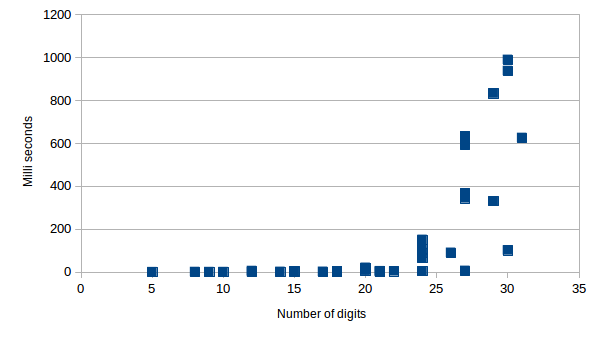
\includegraphics[width=\textwidth]{faktorisera_tider}
\caption{The time to factor a random product of two primes, the x axis represents the number of digits in the product. Each square represents a measured time for a number.}
\label{fig:my_label}
\end{figure}


%\begin{itemize}
%\item sammansatta tal med 10, 20, 30 siffror och jämför tiderna för att faktorisera med de tre (4?) olika metoderna
%\item tal med siffror med många små primtalsfaktorer
%\item tal med få stora primtalsfaktorer (t. ex. produkt av två 5/10/15-siffriga tal)
%\item hur stora tal kan faktorieseras på 10 minuter? (eller annan rimlig tid)
%\item om tid finns: gör diagram som visar hur mycket tid som krävs för tal med 1,2,3,..,n siffror
%\end{itemize}

\section{Final thoughts}
We have demonstrated that it is possible to implement a quick factorisation algorithm in Java, using 64-bit integer arithmetic. One could possibly push the running time down a bit further, by replacing Pollard Rho with a highly optimised 64-bit integer implementation of ECM or by batching GCD computations in Pollard Rho: Instead of calculating \verb!gcd(x_i - x_j, N)! in each iteration, multiply many \verb!x_i - x_j! terms together modulo $N$, and then do one GCD computation, say every 128:th iteration.

Of course a C implementation would probably be faster.

\bibliographystyle{acm}
\bibliography{refs}
\addcontentsline{toc}{section}{Bibliography}
\end{document}
